\documentclass[11pt]{report}

\usepackage{sectsty}
\usepackage{graphicx}
\usepackage{pdfpages}
\usepackage{etoolbox}
\usepackage{hyperref}
\usepackage[backend=biber,style=numeric,sorting=custom,minnames=3, maxnames=6]{biblatex}
\usepackage{minitoc}
\usepackage{fancyhdr}
\usepackage{longtable}

% \usepackage[T1]{fontenc}
% \usepackage[french]{babel}
% \hyphenation{é-chan-tillon-nage}


% Margins
\topmargin=-0.45in
\evensidemargin=0in
\oddsidemargin=0in
\textwidth=6.5in
\textheight=9.0in
\headsep=0.25in

\title{ Demande d'inscription en Habilitation à Diriger des Recherches}
\author{ Mathieu Léonardon }
\date{\today}

% Mettre en pied de page le numéro de page comme ailleurs
\fancypagestyle{includepdfstyle}{
  \fancyhf{}
  \fancyfoot[C]{\thepage}
  \renewcommand{\headrulewidth}{0pt} % Remove top rule
  \renewcommand{\footrulewidth}{0pt} % Remove bottom rule
}

\addbibresource{all.bib}

\DeclareSortingTemplate{custom}{
  \sort{
    \field{sortkey}
  }
}

\begin{document}
\dominitoc % Active les mini-tables des matières

\renewcommand{\contentsname}{
    \begin{center}
    Demande d'inscription en Habilitation à Diriger des Recherches \\ --- \\ Mathieu Léonardon
    \end{center}
    }
\tableofcontents
\vspace{1.5cm}

\section{Experts externes HDR proposés}
\begin{itemize}
    \item Stefan Duffner - \texttt{stefan.duffner@insa-lyon.fr}
    \item Frédéric Pétrot - \texttt{frederic.petrot@univ-grenoble-alpes.fr}
    \item Olivier Sentieys - \texttt{olivier.sentieys@inria.fr}
    \item Andrea Pinna - \texttt{andrea.pinna@lip6.fr}
    \item Nicolas Gac - \texttt{nicolas.gac@universite-paris-saclay.fr}
\end{itemize}

\section{Déclaration sur l'honneur}

Je soussigné, Mathieu Léonardon, déclare sur l'honneur n'avoir pas déposé de demande d'inscription en Habilitation à Diriger des Recherches (HDR) dans un autre établissement que l'Université de Bretagne Occidentale (UBO).
\begin{flushright}
    
\includegraphics[width=0.3\textwidth]{signature.png}
\end{flushright}
\section{Raisons du dépôt à l'UBO}

Je dépose mon dossier d'HDR à l'UBO en raison de mon rattachement au Lab-STICC, dont une partie des membres est affiliée à l'UBO, ainsi que de la proximité géographique entre l'UBO et IMT Atlantique, ce dernier n'étant pas habilité à délivrer ce diplôme.




\pagebreak
\refstepcounter{chapter} % Incrémente le compteur et rend la référence possible
\addcontentsline{toc}{chapter}{\protect\numberline{\thechapter}Curriculum Vitæ}

\refstepcounter{section} % Incrémente le compteur et rend la référence possible
\addcontentsline{toc}{section}{\protect\numberline{\thesection}Résumé du parcours professionnel et activités académiques}



% Inclure pdf main-french.pdf
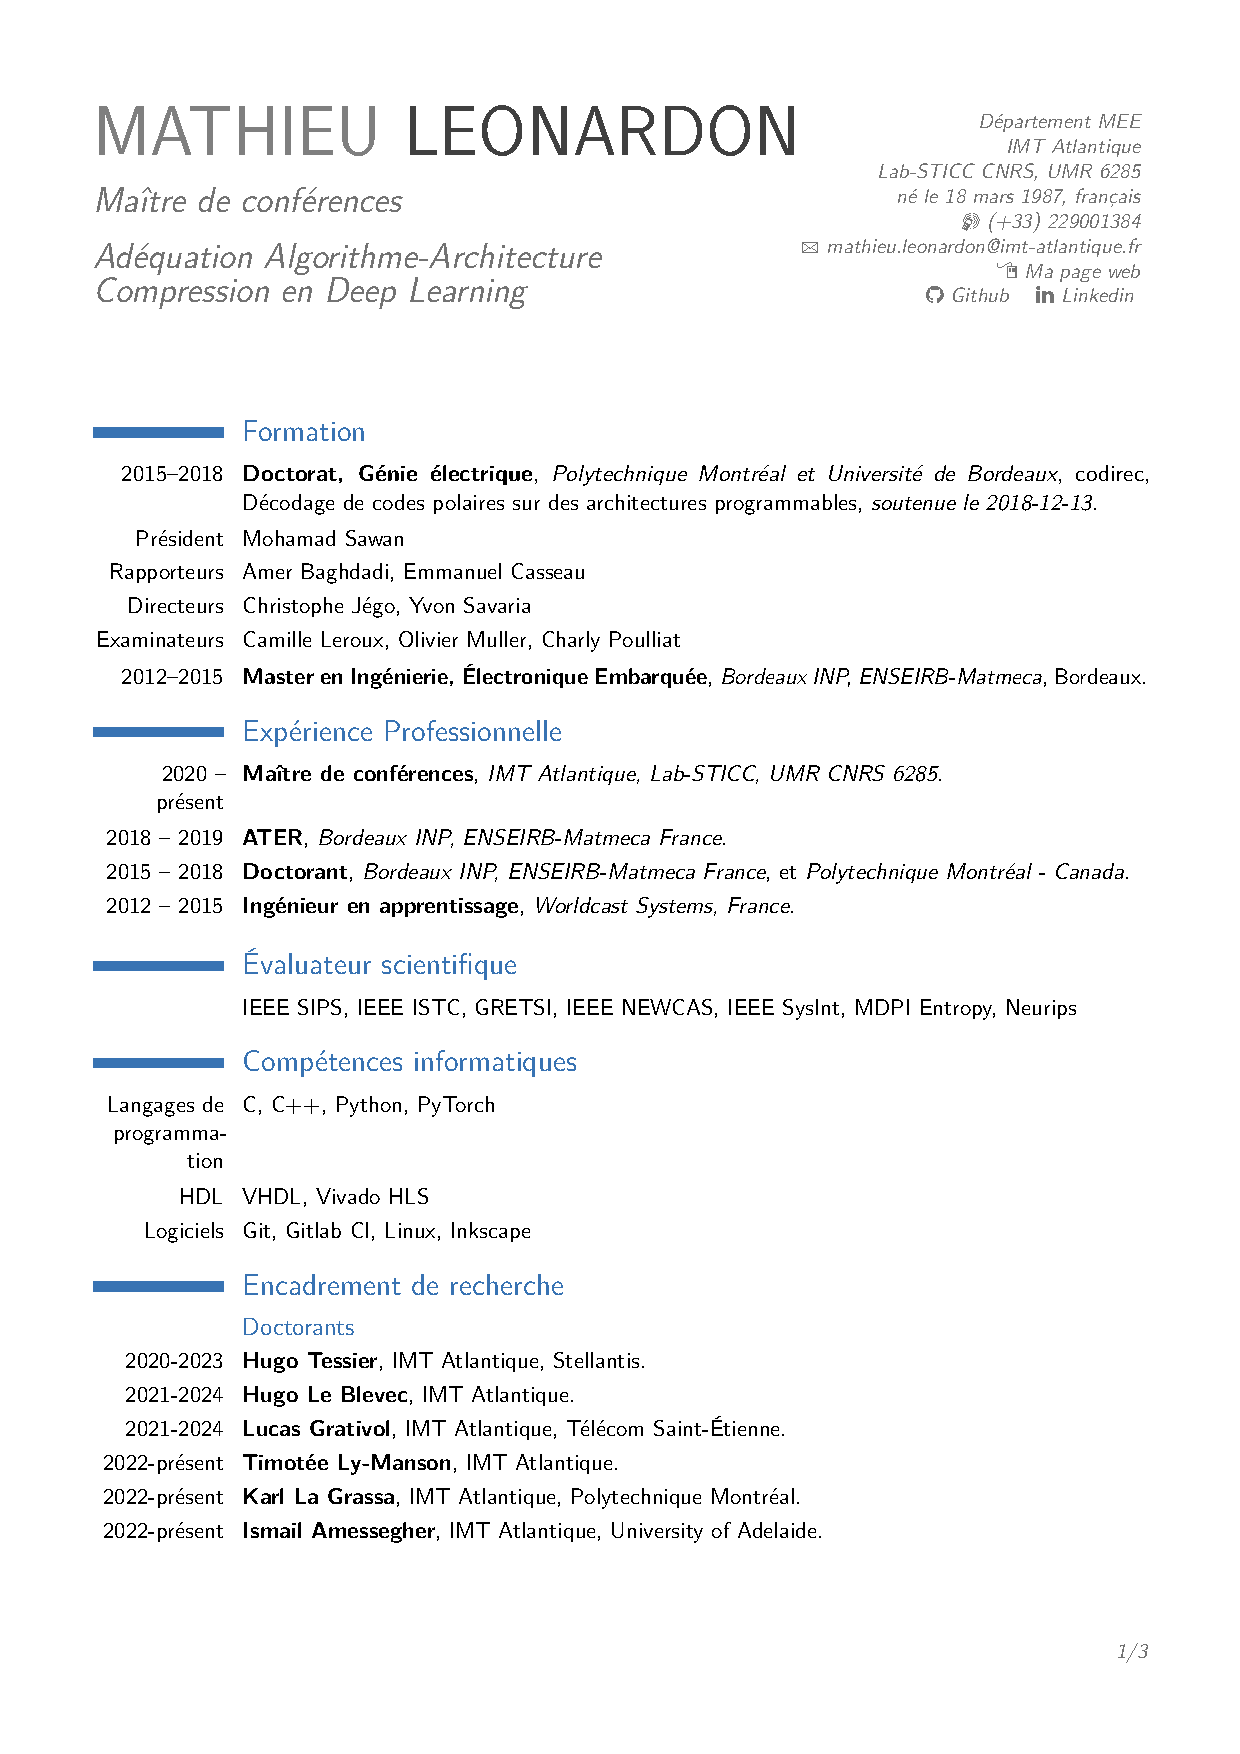
\includepdf[
  pages=-,
  pagecommand={\thispagestyle{includepdfstyle}}
]{main_french.pdf}
\section{Publications}
\subsection{Publications dans des revues internationales}
\printbibliography[keyword={JOURNAL}, heading=none]
\subsection{Publications dans des conférences internationales avec actes}
\printbibliography[keyword={CONFERENCE}, heading=none]
\subsection{Publications dans des conférences nationales avec actes}
\printbibliography[keyword={NATIONAL}, heading=none]
\subsection{Communications sans actes}
\printbibliography[keyword={WORKSHOP}, heading=none]


\pagebreak

\chapter{Résumé des activités de recherche, encadrement et financement}
% \minitoc
% \vspace{1cm}

Ce chapitre présente un résumé des activités de recherche. J'ai réalisé une thèse de doctorat nommée \textit{Décodage de codes polaires sur des architectures programmables}. Poursuivis par un poste d'ATER, ces travaux ont également mené à la création du logiciel open source qui permet la simulation de chaînes complètes de communications numériques ainsi que leur implémentation dans le cadre de radio logicielle (SDR: Software Defined Radio). J'ai ensuite réorienté mes recherches sur la compression d'algorithmes d'apprentissage profond et leur déploiement sur cibles embarquées : FPGA, processeurs et microcontrôleurs embarqués, GPUs embarqués. Mes activités d'encadrement (3 thèses de doctorat soutenues, 4 en cours, 2 post-doctorants, 1 ingénieur de recherche) sont résumées dans la Section~\ref{sec:encadrement}. Enfin, la Section~\ref{sec:financement} liste les financements de recherche obtenus.

\section{Algorithmes de communications numériques sur architectures programmables}
\label{sec:chaines_communication}

Ma thèse de doctorat présente des méthodes d'implémentation efficaces (débit, latence, consommation énergétique) des algorithmes de décodage de code polaires sur des architectures matérielles spécifiques (ASIP: Application Specific Instruction-set Processor) mais également sur des processeurs génériques (GPP: General Purpose Processor). Ces travaux, en collaboration avec Adrien Cassagne du LIP6, ont mené à la création du logiciel open source AFF3CT, une boîte à outil logicielle complète pour la simulation et l'implémentation de chaînes de communication numériques.


\subsection{Décodage de codes polaires sur processeurs génériques}

Les implémentations logicielles des décodeurs de codes correcteurs d'erreurs jouent un rôle crucial dans plusieurs domaines des communications numériques modernes. Premièrement, elles sont essentielles pour les simulations Monte Carlo, permettant d'évaluer les performances des systèmes de communication sous divers scénarios de bruit et d'interférences. Deuxièmement, dans le contexte des réseaux Cloud-RAN (Cloud Radio Access Networks), les décodeurs logiciels offrent la flexibilité nécessaire pour virtualiser les fonctions de la couche physique, facilitant ainsi le traitement coopératif multi-points. Ces décodeurs sont en effet les briques les plus gourmandes en calcul de la chaîne de communication. Enfin, pour les radios logicielles (SDR), elles permettent une reconfiguration dynamique des paramètres de communication, adaptant ainsi les systèmes à différents standards et conditions de canal sans nécessiter de modifications matérielles.

Les codes polaires, introduits par Arıkan en 2009, sont les premiers codes correcteurs d'erreurs à atteindre la capacité de Shannon de manière prouvée pour des longueurs de code infinies. L'algorithme de décodage Successive Cancellation (SC) a été initialement proposé pour les codes polaires, mais sa performance en termes de taux d'erreur binaire (BER) et de taux d'erreur trame (FER) est insuffisante pour les codes de courte longueur. Pour remédier à cela, l'algorithme Successive Cancellation List (SCL) a été proposé dans la littérature, améliorant significativement les performances de décodage en maintenant une liste de chemins candidats. Une version optimisée, appelée Fast SCL, a ensuite été développée pour réduire la complexité computationnelle tout en maintenant une bonne performance de décodage. Ces algorithmes permettent d'atteindre des compromis entre la complexité, la latence et la performance de décodage, rendant les codes polaires adaptés aux standards de communication modernes comme la 5G.

J'ai proposé plusieurs contributions majeures pour l'implémentation logicielle des décodeurs SCL~\cite{leonardon:hal-01987848}. Tout d'abord, un nouvel algorithme de tri partiel est introduit pour optimiser la gestion des chemins candidats dans le décodeur, améliorant ainsi la vitesse de décodage. Ensuite, une nouvelle technique de gestion de la mémoire est proposée pour réduire l'empreinte mémoire et augmenter l'efficacité du décodage. Enfin, une méthode automatisée pour la construction des nœuds de décodage est développée, permettant une implémentation plus flexible et générique des décodeurs. Ces contributions permettent de créer un décodeur logiciel qui est non seulement rapide mais aussi flexible, capable de s'adapter à différents paramètres de code et conditions de canal sans nécessiter une recompilation du code source.

Les résultats présentés dans cet article ont constitué l'état de l'art pour les décodeurs Adaptive SCL sur les GPP du point de vue des débits et de la latence. Près de dix ans après sa publication, les résultats obtenus sont toujours compétitifs. Ces travaux ont été repris à de nombreuses reprises pour être intégrés dans des systèmes plus complexes en limitant le temps et l'énergie consommée par les décodeurs de codes correcteurs d'erreur. Cependant, d'autres algorithmes ont été proposés depuis, comme des améliorations de l'algorithme Successive Cancellation Flip (SCF), qui pourraient bénéficier de techniques similaires pour optimiser leurs performances \cite{Sagitov2025}. Il serait donc intéressant d'explorer ces possibilités dans de futurs travaux pour continuer à améliorer l'efficacité et la flexibilité des décodeurs de codes polaires.

\subsection{La suite logicielle AFF3CT}
Les travaux de recherche menés durant ma thèse ont abouti à la création d'une suite logicielle complète nommée AFF3CT\footnote{\url{https://aff3ct.github.io/}}~\cite{cassagne:hal-02358306,cassagne:hal-01965633}. Cette suite a été conçue pour répondre à plusieurs besoins critiques dans le domaine des communications numériques, notamment en matière de simulations Monte Carlo, de décodage canal, et d'implémentation de systèmes de radio logicielle (SDR).

AFF3CT est un outil puissant pour effectuer des simulations Monte Carlo efficaces et optimisées. Il exploite efficacement les architectures multicœurs et les instructions SIMD (Single Instruction Multiple Data). Les principales briques de la chaîne de communication en bande de base, telles que la source, le codage de canal, la modulation, l'accès multiple~\cite{ghaffari:hal-01977885,ghaffari:hal-03762203}, la démodulation, le décodage de canal, et le monitoring des erreurs, sont toutes disponibles dans AFF3CT. La suite logicielle supporte un grand nombre de codes, de modulations et de canaux, accompagnés d'une documentation exhaustive et détaillée\footnote{\url{https://aff3ct.readthedocs.io}}. Des scripts d'intégration continue sont utilisés pour, lors de chaque nouvelle évolution du logiciel, une base de données complète de courbes BER et FER est rejouée afin d'éviter toute régression dans les modules implémentés.

Les décodeurs de canal d'AFF3CT sont conçus pour être à l'état de l'art ou s'en rapprochant pour les codes polaires, les turbo-codes et les codes LDPC. Un "hall of fame" est disponible sur le site pour chaque type de code, comparant les performances des implémentations disponibles dans AFF3CT avec celles rapportées dans la littérature. Cela permet aux chercheurs et aux ingénieurs de comparer facilement leurs résultats avec les meilleures performances connues, facilitant ainsi l'innovation et l'amélioration continue des algorithmes de décodage.

Suite à ces développements initiaux, j'ai participé, lors de mon année d'ATER, à la transformation d'AFF3CT pour l'adapter à un contexte d'implémentation SDR en utilisant des modules USRP. Cette transformation a permis de rendre AFF3CT compatible avec des systèmes de radio logicielle, ouvrant ainsi la voie à des applications pratiques et réelles dans le domaine des communications numériques. Les principaux résultats de cette transformation incluent une amélioration significative de la flexibilité et de la portabilité du système, permettant une intégration facile avec des équipements matériels variés~\cite{cassagne:hal-03336450}.

Enfin, nous prévoyons de participer, en fin 2025, avec les coauteurs du papier AFF3CT, à la compétition d'implémentation logicielle de la conférence ISTC. Les résultats préliminaires sont très prometteurs et montrent que notre suite logicielle est compétitive par rapport aux autres solutions disponibles. Cette participation nous permettra de valider davantage les performances et la robustesse d'AFF3CT dans un contexte de compétition et de benchmarking international.


\subsection{Architectures ASIP pour les codes polaires}
Dans la continuité des travaux sur les implémentations logicielles de décodage de codes polaires sur processeurs généralistes (GPP), deux contributions ont exploré l'optimisation des performances via des processeurs programmables spécialisés (ASIP - Application Specific Instruction-set Processor). Ce changement de paradigme s'inscrit dans la logique du Cloud-RAN, où la virtualisation des fonctions physiques permet une grande flexibilité d'allocation des ressources. Néanmoins, pour atteindre des objectifs de débit élevé et de sobriété énergétique tout en conservant une certaine programmabilité, le recours aux ASIP se révèle particulièrement pertinent. Contrairement aux GPP, souvent surdimensionnés et énergivores, les ASIP permettent de dimensionner finement les ressources matérielles à l'algorithme cible, tout en intégrant des unités de traitement vectoriel ou des instructions spécifiques pour améliorer l'efficacité.

Le premier travail s'est appuyé sur l'écosystème Cadence Tensilica pour concevoir un processeur basé sur le cœur Xtensa LX7, adapté au décodage SC et SCAN (Soft CANcellation) de codes polaires~\cite{leonardon:hal-03291077}. Ce processeur a été configuré pour inclure un pipeline VLIW, des instructions SIMD sur registres 512 bits, et un ensemble réduit de registres généraux optimisés pour l'accès aux LLR et aux sommes partielles. L'approche a combiné des optimisations architecturales (instructions personnalisées, gestion mémoire adaptée, arithmétique quantifiée) et logicielles (pseudo-unrolling du décodage, usage de fonctions spécialisées type R0/R1/REP/SPC). Les résultats ont montré que le débit était comparable à celui obtenu sur un ARM Cortex-A57, avec une consommation énergétique réduite d'un facteur 10, démontrant ainsi la pertinence de l'approche pour des applications embarquées ou déportées sur des serveurs Cloud-RAN exigeant de fortes contraintes d'efficacité énergétique.

Le second article propose une évolution significative de cette approche via l'utilisation d'une architecture Transport Triggered (TTA), en collaboration avec l'Université de Tampere (qui a également mené à la visite effectuée dans le cadre du projet avec Pekka Jääskeläinen via un financement Maupertuis)~\cite{leonardon:hal-01978830}. Contrairement à l'architecture RISC du LX7, TTA expose explicitement le datapath au compilateur, permettant des transferts directs entre unités fonctionnelles sans passer systématiquement par les registres, ce qui réduit les goulots d'étranglement liés aux accès mémoire. Deux processeurs ont été développés : l'un dédié au SC, l'autre étendu au décodage SCAN. L'architecture TTA s'est avérée particulièrement flexible : l'ajout de fonctions personnalisées (Unrolled SC decoder, unités LLR et PS vectorielles, FUs dédiées à SCAN) s'est effectué sans remise en cause du cœur de compilation. Les résultats sont particulièrement remarquables : un débit de 352 Mbps pour le code (1024, 512), avec une consommation énergétique divisée par 100 (14 nJ/bit) par rapport à une implémentation x86 équivalente. La validation a été menée à la fois sur FPGA (Artix-7) et par synthèse ASIC en 28 nm. Le gain en efficacité énergétique, combiné à une plus grande expressivité pour exprimer les optimisations liées au décodage polaire (notamment le traitement efficace des nœuds spécialisés), positionne les ASIP-TTA comme une solution de compromis particulièrement pertinente entre la rigidité des IP matérielles dédiées et la généricité des GPP.




\section{Apprentissage profond sur cibles embarquées}
\label{sec:deep_learning_embedded}

Mon arrivée à IMT Atlantique en 2020 a marqué le début de mes travaux sur l'apprentissage profond pour les cibles embarquées, avec un accent particulier sur l'optimisation des modèles pour les environnements à ressources limitées.

\subsection{Apprentissage fédéré à faible coût}
Le Federated Learning (FL) est une approche prometteuse pour l'apprentissage automatique distribué, particulièrement adaptée aux applications sensibles à la confidentialité des données, telles que les domaines militaires et médicaux, où les données des clients ne peuvent être partagées ou transférées vers un serveur de cloud computing. Dans le FL standard, un serveur envoie un modèle à un groupe de clients, qui l'entraînent sur leurs données locales, puis renvoient leurs paramètres mis à jour au serveur pour agrégation. Ce processus tente de mieux garantir la confidentialité des données utilisateur, car les données ne quittent jamais l'appareil client.

Cependant, le coût de communication représente un défi majeur dans le FL en raison de son utilisation intensive du réseau. Les appareils clients, comme les smartphones ou les nœuds de l'Internet des Objets (IoT), disposent de ressources limitées en termes d'énergie, de calcul et de mémoire. Pour dépasser ces contraintes matérielles, des modèles légers et des techniques de compression telles que l'élagage (pruning) et la quantification sont couramment adoptées dans les paradigmes centralisés.

Dans une première contribution, nous avons proposé une méthode pour insérer la technique d'élagage en tant qu'étape supplémentaire avant la communication des résultats d'entraînement~\cite{grativol:hal-04251969,grativol:emse-04217775}. Cette approche vise à rendre les messages plus creux (sparse) et ainsi à réduire la taille des messages. Plus précisément, la méthode utilise un élagage non structuré basé sur la magnitude, où les poids avec les plus petites valeurs absolues sont remplacés par des zéros selon un taux d'élagage prédéterminé. Ce processus est effectué par le serveur et les clients avant la transmission d'un message, garantissant un niveau d'élagage équivalent tout au long de chaque tour de communication.

Les résultats démontrent que cette méthode permet de compresser les messages jusqu'à 50 \% tout en entraînant une perte de précision inférieure à 1 \%, surpassant ainsi les techniques de l'état de l'art. Par exemple, avec un taux d'élagage de 50 \%, la taille du message est réduite à 23,0 Mo, avec une précision de 83.85±0.65 \%, contre 44,7 Mo et 84.43±0.36 \% pour le modèle complet sans élagage. Une augmentation du nombre d'itérations locales par client pendant l'entraînement contribue à un modèle plus robuste, permettant des communications de données plus éparses tout en maintenant une précision similaire.

Dans une seconde contribution, nous introduisons FLoCoRA, une méthode qui intègre les techniques LoRA à l'entraînement de modèles de vision de petite taille dans un contexte de federated learning (FL)~\cite{grativol:hal-04617632}. Contrairement aux approches précédentes centrées sur de grands modèles, FLoCoRA adopte une stratégie agnostique à l'agrégation et conserve le modèle de base figé tout au long de l'entraînement. Seuls les paramètres des adaptateurs LoRA, beaucoup plus légers, sont mis à jour et échangés entre les clients. Cette conception permet à la fois de limiter les échanges de données et de réduire l'usage mémoire, grâce à l'absence de calcul et de stockage des gradients du modèle principal.

Les contributions principales incluent : l'intégration d'adaptateurs LoRA dans le cadre du FL, avec une implémentation compatible avec n'importe quelle méthode d'optimisation FL, établissant ainsi une base solide pour la réduction de la communication et de la mémoire; une réduction des tailles de message jusqu'à 4,8 fois avec une perte de précision de moins de 1 \% pour une tâche de classification CIFAR-10 utilisant un ResNet-8; et l'extension de la méthode avec un schéma de quantification affine, permettant des taux de compression encore plus élevés, divisant le coût de communication par 18,6 fois, tout en maintenant une perte de précision inférieure à 1 \% sur un modèle ResNet-18.

Par rapport aux méthodes conventionnelles de compression, FLoCoRA atteint une dégradation de précision moindre pour des messages de taille réduite. Par exemple, pour un taux d'élagage de 40 \% (27,1 Mo) avec la méthode d'élagage par magnitude, la précision est de 85.20±0.20 \%. En revanche, FLoCoRA avec un rang de 64 et quantification à 8 bits (2,4 Mo) atteint 85.24±0.23 \%, représentant une réduction de 18,6 fois le coût de communication par rapport au modèle complet FedAvg (44,7 Mo). L'intégration de la quantification affine a permis de porter la réduction du coût de communication à un facteur 64 avec une perte de précision d'environ 4 \%.

Ces travaux démontrent que LoRA, bien que couramment utilisé pour le fine-tuning, peut servir de base solide pour les économies de communication dans le FL, ouvrant la voie au déploiement du Federated Learning sur des appareils edge où la communication est un goulot d'étranglement et la puissance de calcul est limitée.


\subsection{Compression par élagage ou quantification et déploiement embarqué}

Un autre ensemble de contributions a porté sur l'élagage des réseaux de neurones et ont été menés dans le cadre de la thèse d'Hugo Tessier, en collaboration avec Matthieu Arzel et Vincent Gripon de l'IMT Atlantique, grâce à un financement CIFRE de l'entreprise Stellantis, avec Thomas Hannagan et David Bertrand en tant qu'encadrants.
Une première contribution notable concerne l'élagage efficace des réseaux de neurones via l'application ciblée d'un weight decay à un sous-ensemble de pondérations. Cette méthode, nommée Selective Weight Decay (SWD) ou Pénalisation Sélective des Pondérations (PSP), est décrite dans les articles~\cite{tessier:hal-03675138,tessier:hal-03695958}. Inspirée du lissage Lagrangien, la PSP permet un élagage progressif et continu durant l'entraînement. Elle repose sur l'ajout d'un terme de pénalité dans la fonction objectif, avec un coefficient $a$ croissant exponentiellement entre $a_{min}$ et $a_{max}$. Ce schéma garantit un entraînement initial non perturbé, suivi d'un élagage efficace des connexions lorsque $a_{max}$ est suffisamment élevé.
La PSP s'applique aussi bien à l'élagage non structuré (réduction des pondérations de faible norme à zéro) qu'à l'élagage structuré (suppression de canaux entiers via les coefficients multiplicatifs des couches de normalisation).

Les résultats montrent une efficacité particulière pour les taux d'élagage élevés, où les approches classiques dégradent fortement les performances. Sur des jeux de données comme CIFAR-10 et ImageNet ILSVRC2012, la PSP surpasse les méthodes de référence. Sa robustesse et sa transposabilité sont appuyées par une revue approfondie de la littérature. Un article de blog à bon impact a également vulgarisé cette approche\footnote{\url{https://towardsdatascience.com/neural-network-pruning-101-af816aaea61/}}.

L'élagage de modèles plus complexes, comme ceux dédiés à la segmentation sémantique, présente toutefois des défis spécifiques pour obtenir des gains tangibles sur cibles embarquées, notamment en raison d'incohérences dimensionnelles entre couches. Des solutions ont été proposées pour exploiter l'élagage structuré global tout en évaluant son impact réel sur la consommation énergétique sur GPU embarqué.
La méthode proposée résout ces problèmes en identifiant d'abord toutes les parties du réseau qui sont déconnectées lors de la suppression des filtres, en tenant compte de toutes les dépendances architecturales~\cite{tessier:hal-03706472}. Elle adapte ensuite automatiquement les opérations d'addition pour gérer les tenseurs de différentes dimensions, ce qui garantit que tous les filtres et noyaux contribuent à la fonction du réseau, permettant ainsi une mesure plus fiable du taux d'élagage réel et de la complexité associée des réseaux élagués. En particulier, les additions à la fin de chaque bloc résiduel dans les architectures comme ResNet ou HRNet nécessitent que les deux tenseurs d'entrée aient les mêmes dimensions, ce qui peut être résolu en remplaçant les additions par une nouvelle opération "indexation-addition".

Les expériences menées avec cette approche sur des GPU embarqués NVIDIA Jetson AGX Xavier ont démontré que l'élagage structuré global peut réduire la consommation d'énergie. Cependant, il a été constaté que les réseaux plus petits et non élagués, tels que HRNet-32 et HRNet-18, sont plus efficaces énergétiquement que les réseaux élagués, même à nombre d'opérations égal. Cela est attribué à la nature non conventionnelle des opérations d'insertion (ScatterND) utilisées pour gérer les dimensions, qui peuvent nuire à l'optimisation du reste du réseau~\cite{tessier:hal-03767634,tessier:hal-03767636}. Ces résultats soulignent la nécessité d'élaborer une implémentation plus efficace des opérateurs nécessaires pour exploiter l'élagage et d'explorer davantage les biais des critères d'élagage, car ils peuvent conduire à des distributions de sparsité sous-optimales sur le plan énergétique.

En outre, d'autres instances d'amélioration des performances par élagage et quantification ont été explorées. Un projet industriel, mené en collaboration avec l'entreprise GoodFloow, a permis d'étudier l'interopérabilité des techniques de compression (élagage, quantification et codage) pour le déploiement de réseaux de neurones convolutionnels sur des microcontrôleurs à mémoire limitée~\cite{younes:hal-03850858}. Ces travaux ont développé une méthodologie pour optimiser le compromis entre la précision du modèle et l'empreinte mémoire, crucial pour les applications. Parallèlement, des recherches ont porté sur l'utilisation de technologies émergentes basées sur les memristors pour l'élaboration de réseaux de neurones binaires~\cite{alhajali:hal-03659297}. Ces approches de "calcul in-memory" visent à surmonter le goulot d'étranglement des données en effectuant des calculs directement au sein de la mémoire, offrant des gains significatifs en vitesse et en efficacité énergétique pour les réseaux de neurones binaires, particulièrement bien adaptés à ces technologies. De plus, des développements d'implémentations SIMD (Single Instruction Multiple Data) pour les réseaux de neurones convolutionnels sur processeurs à usage général (GPP) ont été réalisés en collaboration avec la startup canadienne Deeplite~\cite{ganji:hal-04082069}. Ce projet, appelé DeepGEMM, s'est basé sur une utilisation de tables de correspondance (LUT) implémentées à l'aide des jeux d'instructions Intel AVX2 et Arm Neon.

\subsection{Apprentissage profond sur cibles FPGA}
Les travaux de thèse d'Hugo Le Blevec se sont concentrés sur la co-conception de réseaux de neurones profonds et d'architectures FPGA en pipeline pour la segmentation sémantique dans le cadre des véhicules autonomes~\cite{leblevec:hal-04262138,leblevec:hal-04705594}. Ces systèmes exigent une faible latence et une consommation réduite, ce qui rend les GPU classiques peu adaptés en contexte embarqué. Les FPGA offrent une alternative prometteuse grâce à leur traitement parallèle et leur efficacité énergétique, bien qu'ils posent des défis liés aux ressources limitées.

La thèse a mis en lumière l'impact souvent sous-estimé des routines d'entraînement. En optimisant celles-ci sur un modèle léger comme ENet, des gains de plus de 12 \% sur Cityscapes et 26 \% sur CamVid ont été obtenus. Cela démontre qu'un entraînement soigné permet à des architectures simples de rivaliser avec des modèles plus complexes.
L'architecture ENet a ensuite été adaptée pour un mappage efficace sur FPGA, en s'appuyant sur le framework open-source FINN. Des contributions notables incluent l'ajout de transformations de streamlining et l'intégration des convolutions transposées, indispensables pour la segmentation. Le modèle final, P-ENet, atteint 70.3 \% de mIoU en INT4, avec 4.2 ms de latence et 226 FPS sur Cityscapes. Il surpasse les implémentations FPGA existantes et se révèle 1.15 fois plus efficace énergétiquement qu'une NVIDIA Jetson AGX Xavier. Ces travaux ne sont pour présentés dans le manuscrit, mais en cours de soumission à ACM TRETS.

En parallèle, le projet PEFSL (Pipeline for Embedded Few-Shot Learning), issu d'un projet étudiant que j'ai encadré, lauréat du concours OpenHardware AMD Xilinx 2023\footnote{https://www.openhw.eu/2023-results-gallery}, s'est attaqué à l'apprentissage few-shot sur FPGA-SoC. Le flot développé, basé sur Tensil, couvre l'ensemble de l'entrainement, de la chaîne de conception et du déploiement sur une carte PYNQ-Z1. Le démonstrateur atteint une latence de 30 ms pour une consommation de 6.2 W sur MiniImageNet~\cite{grativol:hal-04559365}.

Ce travail a conduit à une collaboration avec l'université de Tohoku et le professeur Naoya Onizawa, concrétisée par des visites croisées et deux publications~\cite{kanda:hal-04984380,kanda:hal-04984381}. Ces articles visent à assurer la cohérence de la précision tout au long du flux de conception, en appliquant la quantification en virgule fixe via Brevitas, avec des méthodes QAT et PTQ. Ils montrent qu'une précision proche de celle en virgule flottante peut être atteinte avec seulement 5 à 6 bits pour les parties entières et fractionnaires. Ces modèles ont ensuite été intégrés dans la suite FINN au sein de PEFSL.
\section{Résumé des activités d'encadrement}
\label{sec:encadrement}

\subsection{Encadrement de doctorants}
Thèses soutenues :
\begin{itemize}
    \item Hugo Tessier, soutenue le 09/02/2023
    \item Lucas Grativol Ribeiro, soutenue le 05/12/2024
    \item Hugo Le Blevec, soutenue le 06/12/2024
\end{itemize}
Thèses en cours :
\begin{itemize}
    \item Timotée Ly-Manson, soutenance prévue en décembre 2025
    \item Ismail Amessegher, soutenance prévue en décembre 2025
    \item Jérémy Morlier, soutenance prévue en décembre 2026
    \item Elise Lagarde, depuis janvier 2025
\end{itemize}
\subsection{Encadrement de stages de master}
\begin{itemize}
    \item Hugo Kermabon, de mai à août 2020
    \item Hugo Le Blevec, de avril à octobre 2020
    \item Jérémy Morlier, de juin à juillet 2021
    \item Lubin Gauthier, de juillet à septembre 2023
    \item Pedro Figueireido, de mai à aout 2025
    \item Mohammed El Houcine Ayoubi, de avril à aout 2025
\end{itemize}
% \small % Réduit la taille de la police pour tout le tableau
% \begin{longtable}{|p{0.25\linewidth}|p{0.13\linewidth}|c|p{0.18\linewidth}|c|p{0.15\linewidth}|}
% \caption{Activités d'enseignement} \label{tab:activites_enseignement} \\
% \hline
% \textbf{Nom de l'enseignement} & \textbf{Membre ou Lead} & \textbf{HETD} & \textbf{\'Etablissement} & \textbf{Ann\'ee scolaire} & \textbf{Niveau} \\
% \hline
% \endfirsthead
% \hline
% \textbf{Nom de l'enseignement} & \textbf{Membre ou Lead} & \textbf{HETD} & \textbf{\'Etablissement} & \textbf{Ann\'ee scolaire} & \textbf{Niveau} \\
% \hline
% \endhead
% \hline
% \endfoot
% \hline
% \endlastfoot
% Projet de conception en \'electronique & Lead & 50.00 & ENSEIRB-MATMECA & 2015-2020 & L3\\
% Architecture reconfigurable & Lead & 20.00 & ENSEIRB-MATMECA & 2015-2020 & M1\\
% \'Electronique Num\'erique & Lead & 25.00 & ENSEIRB-MATMECA & 2015-2020 & L3\\
% Logique combinatoire et logique s\'equentielle & Membre & 32.00 & ENSEIRB-MATMECA & 2015-2020 & L3\\
% Projet micro-processeur & Membre & 36.00 & ENSEIRB-MATMECA & 2015-2020 & L3\\
% Architecture des ordinateurs & Membre & 16.00 & ENSEIRB-MATMECA & 2015-2020 & M1\\
% Projet micro-informatique & Membre & 42.00 & ENSEIRB-MATMECA & 2015-2020 & M1\\
% Programmation objet. Langage C++ & Membre & 15.00 & ENSEIRB-MATMECA & 2015-2020 & M1\\
% Conception haut niveau de circuits & Membre & 46.25 & IMT Atlantique & 2020-2025 & M1-M2\\
% Efficient Deep Learning & Lead & 300.00 & IMT Atlantique & 2020-2025 & M1-M2\\
% Electronique & Membre & 88.75 & IMT Atlantique & 2020-2025 & L3\\
% Architecture des ordinateurs & Lead & 31.25 & IMT Atlantique & 2020-2025 & L3\\
% Fonctions electroniques logiques et analogiques & Membre & 13.75 & IMT Atlantique & 2020-2025 & L3\\
% Calcul parall\'ele pour l'ing\'enieur & Lead & 137.50 & IMT Atlantique & 2020-2025 & M1-M2\\
% Projets divers & Membre & 246.25 & IMT Atlantique & 2020-2025 & L3-M2\\
% M\'ethodologies de conception & Membre & 11.25 & IMT Atlantique & 2020-2025 & M1-M2\\
% Syst\'emes embarqu\'es - interaction hw \textbackslash{} sw & Membre & 132.50 & IMT Atlantique & 2020-2025 & M1-M2\\
% Syst\'emes embarqu\'es : du capteur au traitement intelligent & Membre & 45.00 & IMT Atlantique & 2020-2025 & M1-M2\\
% \end{longtable}

\section{Financement de la recherche}
\label{sec:financement}

\subsection{Financements publics}
{\small
\begin{longtable}{|c|l|p{3cm}|p{1.cm}|p{1.5cm}|}
\caption{Financements publics} \label{tab:financements_publics} \\
\hline
\textbf{Ann\'ee} & \textbf{Titre court} & \textbf{Organisme} & \textbf{R\^ole} & \textbf{Montant (k€)} \\
\hline
\endfirsthead
\endfoot
\hline
\endlastfoot
2023-2027 & Autonomous Pack & ADEME Logistique 4.0& PI & 260 \\
2024-2026 & GNSS Anti-Jamming w/ CRPA \& CNN/TCN & R\'egion Bretagne & co-PI & 140 \\
2023-2026 & ProPruNN: Pruning Neural Networks & ANR JCJC& PI & 250 \\
2023-2026 & Vortex: Drone Swarms for Exploration & ANR TSIA & co-PI & 200 \\
2024-2025 & Deep-Learning-FPGA-Eco-conception & CNES & PI & 5 \\
2021-2025 & GoodFloow & ADEME Perfecto & PI & 70 \\
2022-2024 & Leasard: Low Energy DNN for Drones & Labex CominLabs & co-PI & 120 \\
2022-2024 & FLCNNFPGA: Federated Learning & CNRS GDR ISIS & co-PI & 7 \\
2021-2024 & FLCNNFPGA: Federated Learning \& FPGA & IMT Futur \& Ruptures & co-PI & 120 \\
\end{longtable}
}

\subsection{Financements privés}
{\small
\begin{longtable}{|c|l|p{3cm}|p{1cm}|p{1.5cm}|}
\caption{Financements privés} \label{tab:financements_prives} \\
\hline
\textbf{Ann\'ee} & \textbf{Titre court} & \textbf{Organisme} & \textbf{R\^ole} & \textbf{Montant (k€)} \\
\hline
\endhead
\hline
\endfoot
\hline
\endlastfoot
2025-2028 & GNSS Anti-Jamming Opt. (CIFRE) & Arkane & co-PI & pvt \\
2023-2025 & Few-Shot NAS in Metric-Driven Fmwk & Sony & co-PI & 180k€ \\
2024-2025 & Embedded DL for Seg. \& LLMs & Schneider Electric & PI & 40k€ \\
2020-2023 & CNN Pruning for Embedded Vision (CIFRE) & Stellantis & co-PI & pvt \\
2022 & DeepGEMM: Low-Precision Inference & Deeplite & PI & 60k€\\
\end{longtable}
}
% \minitoc
% \vspace{1cm}
\clearpage
\section{Nouvelles méthodes et architectures pour les codes canal}
\subsection{Intérêt pour les codes courts, pertinence des codes polaires}

Actuellement, les implémentations logicielles de codes correcteurs d'erreur sont très recherchées. Elles offrent une grande flexibilité et réduisent les coûts de développement et de déploiement par rapport aux solutions matérielles dédiées. Je projette actuellement de collaborer avec l'ETS Montréal pour implémenter l'algorithme \textit{Generalized Restart Mechanism} (GRM) \cite{Sagitov2025}. Le GRM réduit le temps d'exécution moyen des décodeurs en sautant les calculs identiques entre les essais de décodage. Cette technique, applicable au Successive-Cancellation Flip (SCF) et au Fast-SCF, diminue le temps d'exécution de 25\% à 60\% sans dégrader la correction d'erreurs, avec seulement 4\% de mémoire additionnelle. Pour sa mise en œuvre, des techniques d'optimisation logicielle comme l'unrolling et la vectorisation seront utilisées. Les résultats préliminaires montrent que les gains en débit et surtout en latence maximum, point faible de l'algorithme Adaptive SCL, sont très significatifs.

Ces développements pourraient s'étendre aux codes polaires quantiques. Le décodeur Successive Cancellation List (SCL) est adaptable aux codes polaires quantiques, offrant des performances élevées et une faible complexité \cite{Gong2024}. Une nouvelle construction de codes polaires quantiques basée sur la polarisation de poids (PW) élimine le besoin d'assistance d'intrication. Le décodeur SCL-C, est pour l'instant basé sur l'algorithme liste. Il serait possible de l'adapter au GRM-SCF, et de réduire ainsi grandement la complexité, jusqu'à une implémentation logicielle complète. Nous avons aussi des possibilités de collaboration sur le sujet de la construction de codes polaires adaptés au décodage SCF à l'aide d'apprentissage profond, à la manière de travaux que j'ai présentés à la conférence ISTC 2023~\cite{leonardon:hal-03291030}.

\subsection{Architectures RISC-V pour décodage de code canal}

Pour le domaine de l'embarqué, il existe de très bonnes raisons d'explorer les architectures RISC-V, un jeu d'instructions (ISA) ouvert et libre, ce qui contraste avec les architectures propriétaires comme ARM ou x86. Cette ouverture permet aux concepteurs de puces et aux développeurs de systèmes de personnaliser l'architecture pour des applications spécifiques sans payer de frais de licence, offrant ainsi une flexibilité et une innovation accrues.
L'un des avantages majeurs de RISC-V pour l'embarqué est sa modularité. Il permet d'ajouter des extensions personnalisées, ce qui est idéal pour les charges de travail spécialisées, comme le décodage de codes correcteurs d'erreurs. Cela signifie qu'il est possible de concevoir un processeur avec des instructions spécifiques qui accélèrent directement les opérations de décodage, conduisant à une meilleure performance et efficacité énergétique que ce qui serait possible avec une architecture générique.

De plus, l'écosystème RISC-V est en pleine croissance, avec un soutien croissant de l'industrie et du monde universitaire. Cela favorise le développement d'outils, de logiciels et de matériels qui facilitent la conception et le déploiement. L'aspect open source de RISC-V encourage également la transparence et la sécurité, des éléments cruciaux pour les systèmes embarqués critiques.

Dans cette optique, j'envisage de collaborer avec Adrien Cassagne du LIP6 (pour les aspects accélération logicielle) et Camille Leroux (accélération matérielle) de Bordeaux INP pour monter une ANR collaborative (PRC) axée sur la conception d'architectures RISC-V spécialisées pour le décodage de codes correcteurs d'erreurs. Cette initiative viserait à exploiter pleinement le potentiel de personnalisation de RISC-V pour créer des solutions embarquées hautement optimisées et performantes.

\section{Spécialisation de réseaux pour cibles embarquées}

Comme montré précédemment, de nombreuses contributions ont été faites dans le domaine de l'apprentissage profond sur cibles embarquées, notamment en ce qui concerne la compression des modèles et leur déploiement sur des architectures matérielles spécifiques. Ces travaux motivent de nouveaux développements. D'une part, leur application dans des domaines spécifiques notamment leur utilisation dans un contexte de brouillage de signaux dans des lanceurs ou le traitement de signaux EEG. D'autre part, la nécessité de prendre un peu de hauteur est de trouver des approches plus systématiques pour la conception de modèles d'apprentissage profond adaptés aux contraintes des cibles embarquées, notamment en utilisant des techniques de co-design entre les modèles et les architectures matérielles à base de NAS (Neural Architecture Search).

\subsection{Application de l'apprentissage profond pour le débruitage GNSS dans un cadre spatial}
À la suite de plusieurs travaux réalisés dans le cadre de contrats de recherche précédents avec l'entreprise Arkane, une problématique centrale s'est dégagée : la vulnérabilité persistante des systèmes de navigation par satellite (GNSS) face aux interférences, brouillages et autres formes de dégradation du signal. Ces constats ont conduit à la définition d'un projet de thèse CIFRE dont l'objectif est de proposer des solutions innovantes pour améliorer la résilience de ces systèmes, en particulier dans des contextes critiques comme les environnements spatiaux ou les applications embarquées à fortes contraintes.

Le projet s'intéresse en particulier aux antennes à réception contrôlée (CRPA), capables de traiter spatialement les signaux pour atténuer les perturbations. Cependant, les méthodes classiques de formation de voie, bien que puissantes sur le plan théorique, restent coûteuses en calcul et peu adaptées aux contraintes de l'embarqué. Pour dépasser ces limites, le travail proposé explore l'intégration du Deep Learning, et notamment de modèles convolutifs, afin de simplifier et d'accélérer les traitements spatio-temporels réalisés par ces antennes.

L'un des défis majeurs du projet réside dans l'adaptation de ces modèles à des plateformes matérielles contraintes, telles que les FPGA, souvent utilisés dans les systèmes embarqués pour leur faible consommation énergétique, leur capacité de reconfiguration, le fait qu'ils sont qualifiés pour l'espace, et la fiabilité de leur approvisionnement. Il s'agira donc de concevoir des architectures de réseaux de neurones à la fois efficaces, compactes et interprétables, permettant une exécution en temps réel sans compromettre la qualité du positionnement, de la synchronisation ou de la vitesse estimée. Des efforts particuliers seront également consacrés à la quantification des modèles, à la réduction de leur complexité, et à l'optimisation de leur déploiement sur le matériel cible.

L'approche adoptée sera résolument interdisciplinaire, en s'appuyant sur des échanges continus entre l'entreprise et une autre équipe de recherche impliquée de Télecom Paris (Comelec). Le projet prévoit une alternance entre phases de conception algorithmique, prototypage, implémentation matérielle et validation expérimentale. Des tests seront menés à la fois en simulation et sur bancs de test réels, afin d'évaluer de manière rigoureuse la robustesse et les performances des solutions proposées dans des environnements représentatifs.

Au-delà des avancées scientifiques attendues, ce travail vise également à produire des résultats concrets et valorisables, que ce soit sous la forme de démonstrateurs embarqués, de publications, ou de dépôts de brevet. L'un des débouchés envisagés concerne l'amélioration des capacités de navigation autonome à bord de lanceurs spatiaux, un domaine d'application déjà exploré dans les travaux antérieurs et pour lequel les perspectives de transfert technologique sont prometteuses.

\subsection{Couches d'attention sur cibles microcontrôleurs pour le traitement de données EEG}

Un projet en cours de structuration au sein de l'équipe BRAIN s'intéresse à l'application des Transformers au traitement en temps réel des signaux électroencéphalographiques (EEG) dans des environnements embarqués. Les architectures de type Transformer ont récemment montré de très bonnes performances pour analyser les données EEG, notamment en raison de leur capacité à capturer des dépendances longues dans les signaux multicanaux~\cite{tegon2025}. Cette orientation méthodologique est de plus en plus présente dans la littérature, mais reste encore peu explorée en contexte de déploiement embarqué.

Une spécificité notable des travaux en EEG est l'utilisation de longues séquences temporelles, souvent nécessaires pour capter les rythmes cérébraux ou des événements discrets. Cela constitue un défi majeur pour l'embarqué, car la complexité des Transformers croît rapidement avec la longueur des séquences. En revanche, contrairement à ce qu'on observe en traitement du langage ou de l'image, les modèles EEG utilisent des architectures relativement compactes, ce qui rend leur exécution sur microcontrôleur envisageable, à condition d'un travail d'optimisation ciblé.

L'objectif du projet est de concevoir un démonstrateur de traitement embarqué en temps réel basé sur des Transformers optimisés pour l'EEG. Cela implique une co-conception matériel-logiciel rigoureuse : maîtrise de l'empreinte mémoire, vectorisation des opérations pour tirer parti des architectures parallèles des microcontrôleurs, et adaptation des couches du modèle aux contraintes matérielles. Une collaboration est prévue avec Giulia Lioi, afin d'assurer la pertinence des méthodes et tâches envisagées et d'ancrer le projet dans des cas d'usage concrets. Ce travail pourrait déboucher sur des dispositifs légers, autonomes et capables de traitements EEG localisés, avec des applications potentielles en neurotechnologie, en diagnostic portable ou en interfaces cerveau-machine.

\subsection{Co-conception de réseaux de neurones et architectures matérielles embarquées}

Enfin, une amélioration possible de mes travaux actuels réside dans le fait que la conception des architectures est réalisée manuellement. Le Neural Architecture Search (NAS) est une approche bien connue et fréquemment citée pour l'automatisation de la conception d'architectures de réseaux de neurones. Cependant, ce domaine est souvent perçu comme déconnecté des réalités pratiques, produisant des architectures qui ne sont pas toujours optimisées pour les contraintes du monde réel.

Les zero-cost proxies (ZCPs), qui permettent le NAS à faible coût en évitant l'entraînement complet des modèles, présentent une limitation fondamentale~\cite{lymanson:hal-04576139}. Bien qu'ils montrent une forte corrélation avec les performances des modèles sur l'ensemble des espaces de recherche, celle-ci diminue drastiquement lorsque l'on se concentre sur les meilleures architectures. Les ZCPs ont tendance à être biaisés vers des architectures ayant un grand nombre de paramètres, ce qui réduit leur pouvoir discriminant pour les modèles de haute performance. Cette faiblesse est particulièrement notable lorsque l'espace de recherche est réduit aux 1 \% des meilleures architectures, où la corrélation entre les ZCPs et la performance réelle chute de manière significative.

Pour pallier ce problème, mon objectif est de développer des techniques plus pragmatiques permettant de concevoir automatiquement des architectures de réseaux de neurones légères, qu'il s'agisse de Transformers ou de CNN. Des travaux préliminaires dans cette direction ont déjà été réalisés. Nous nous concentrons actuellement sur des techniques de sampling sur des supernets, guidées par des métriques zero-shot, afin d'automatiser cette conception de manière plus efficace et adaptée aux contraintes d'implémentation. Le nombre de paramètres du modèle est considéré comme une métrique discriminante simple mais universelle pour contraindre l'espace de reche rche, ciblant ainsi des régions plus adaptées pour une exploration guidée par les ZCPs. Cette approche vise à améliorer la qualité des architectures découvertes, en particulier pour les ZCPs qui peinent à trouver des régions performantes de l'espace par eux-mêmes, et permet de contrôler la taille des modèles échantillonnés, évitant ainsi de surparamétrer les architectures.

De manière similaire, une technique efficace pour la conception de modèles de réseaux de neurones par NAS est le paradigme de Supernet. Il s'agit d'entraîner un modèle de réseau de neurones englobant une grande variété d'architectures possibles, permettant ainsi de découvrir des modèles performants sans avoir à entraîner chaque architecture individuellement. Une des problématiques est de savoir comment effectuer l'entrainement pour qu'à la fin, des sous-réseaux soient capables de fonctionner de manière autonome. Dans la plupart des méthodes, une sélection des sous réseaux à agglomérer à la loss est effectuée, mais cette sélection est réalisée de manière aléatoire. Nous pourrions à la place se focaliser sur des architectures que l'on sait performantes, par exemple en utilisant des zero-cost proxies. Ou alors d'utiliser des modèles experts sur l'adéquation des sous-réseaux à des architecture matérielles données. L'outil Stream développé par l'équipe MICAS de l'Université de Louvain permet par exemple cette modélisation~\cite{symons2022}. Nous avons pris contact avec cette équipe et Jérémy Morlier, doctorant dans le cadre de mon projet JCJC ProPruNN, a commencé à travailler sur l'intégration de Stream dans le cadre de la recherche de sous-réseaux pour des architectures matérielles spécifiques. Une mobilité à l'automne 2025 est prévue pour approfondir cette collaboration et explorer les possibilités offertes par Stream dans le contexte de la recherche de sous-réseaux adaptés aux contraintes matérielles.

\section{Références}
\printbibliography[keyword={REFERENCE}, heading=none]

\end{document}